\documentclass[a4paper,11pt]{article}
\usepackage[utf8]{inputenc}
\usepackage{graphicx}
\usepackage{hyperref}
\usepackage[fontset=mac]{ctex}
\usepackage{amsmath}
\usepackage{amssymb}
\usepackage{listings}
\usepackage{xcolor}
\usepackage{graphicx}
\usepackage{amsmath}
\usepackage{amsfonts}
\usepackage{xcolor}  % 颜色控制包
\title{说明文档:AnaClock-React}
\date{}

\begin{document}

\maketitle

\tableofcontents
\newpage
\section{实现思路}
\section{使用说明}
\subsection{简介}
本应用包含时钟、闹钟、计时器、秒表以及明暗模式切换功能。

\subsection{时钟}
\subsubsection{表盘}
如图\ref{fig:clock}所示,在时钟界面中含有指针式表盘以及数字式表盘,两个表盘的时间总是保持一致

其中在指针式表盘中含有时针、分针和秒针(秒针按照要求设计为红色),支持秒针在刻度之间平滑移动。
\begin{figure}[!h]
    \centering
    \begin{minipage}{0.7\textwidth}
        \centering
        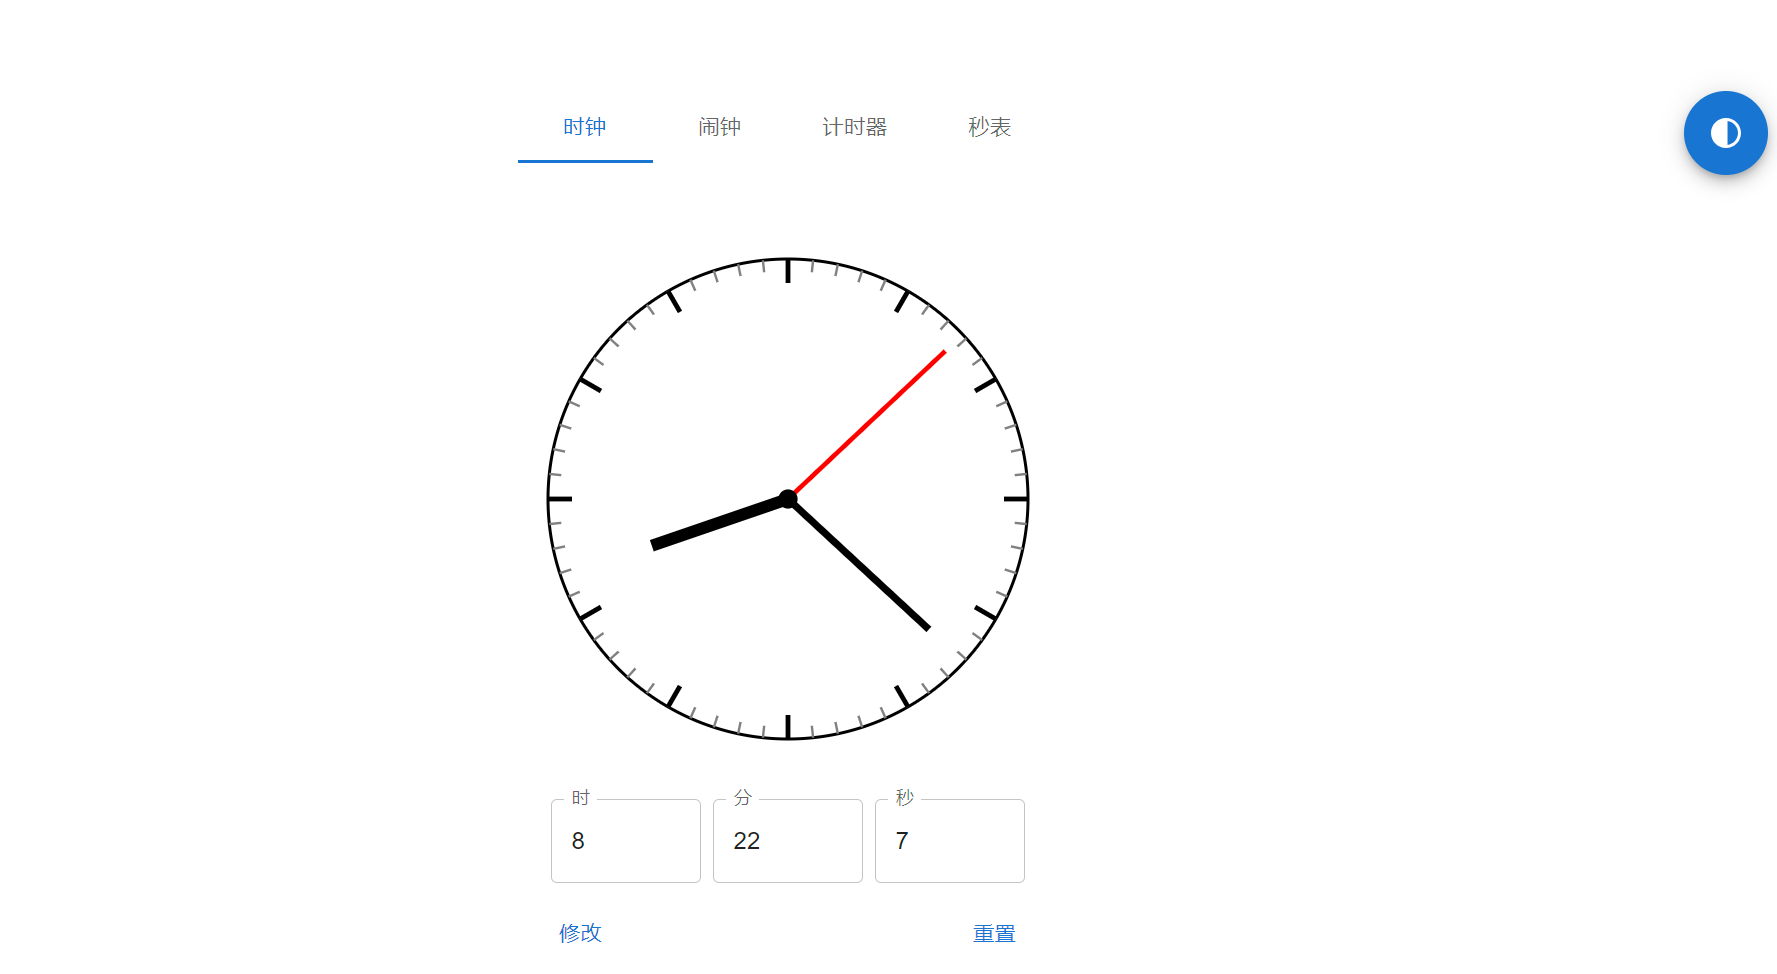
\includegraphics[width=\linewidth]{image/clock.png}
        \caption{clock}
            \label{fig:clock}
    \end{minipage}
\end{figure}
\subsubsection{更改时间}
在图\ref{fig:clock}中可支持通过指针式表盘或是数字式表盘更改时间:
\begin{itemize}
  \item 指针式表盘:可直接通过鼠标拨动时针、分针和秒针来更改时间;
  \item 数字式表盘:可通过点击“修改”,再直接在数字式表盘中更改时间。
  \item 点击“重置”后可使两个表盘时间回到显示北京时间。
\end{itemize}

\subsection{闹钟}

\subsubsection{添加闹钟}
在图\ref{fig:alarm}中,点击“+”按钮后进入图\ref{fig:alarm_add},进行添加闹钟操作,在确定好时间后,点击“确认”即可在右方看到设置的闹钟。
\begin{figure}[!h]
    \centering
    \begin{minipage}{0.48\textwidth}
        \centering
        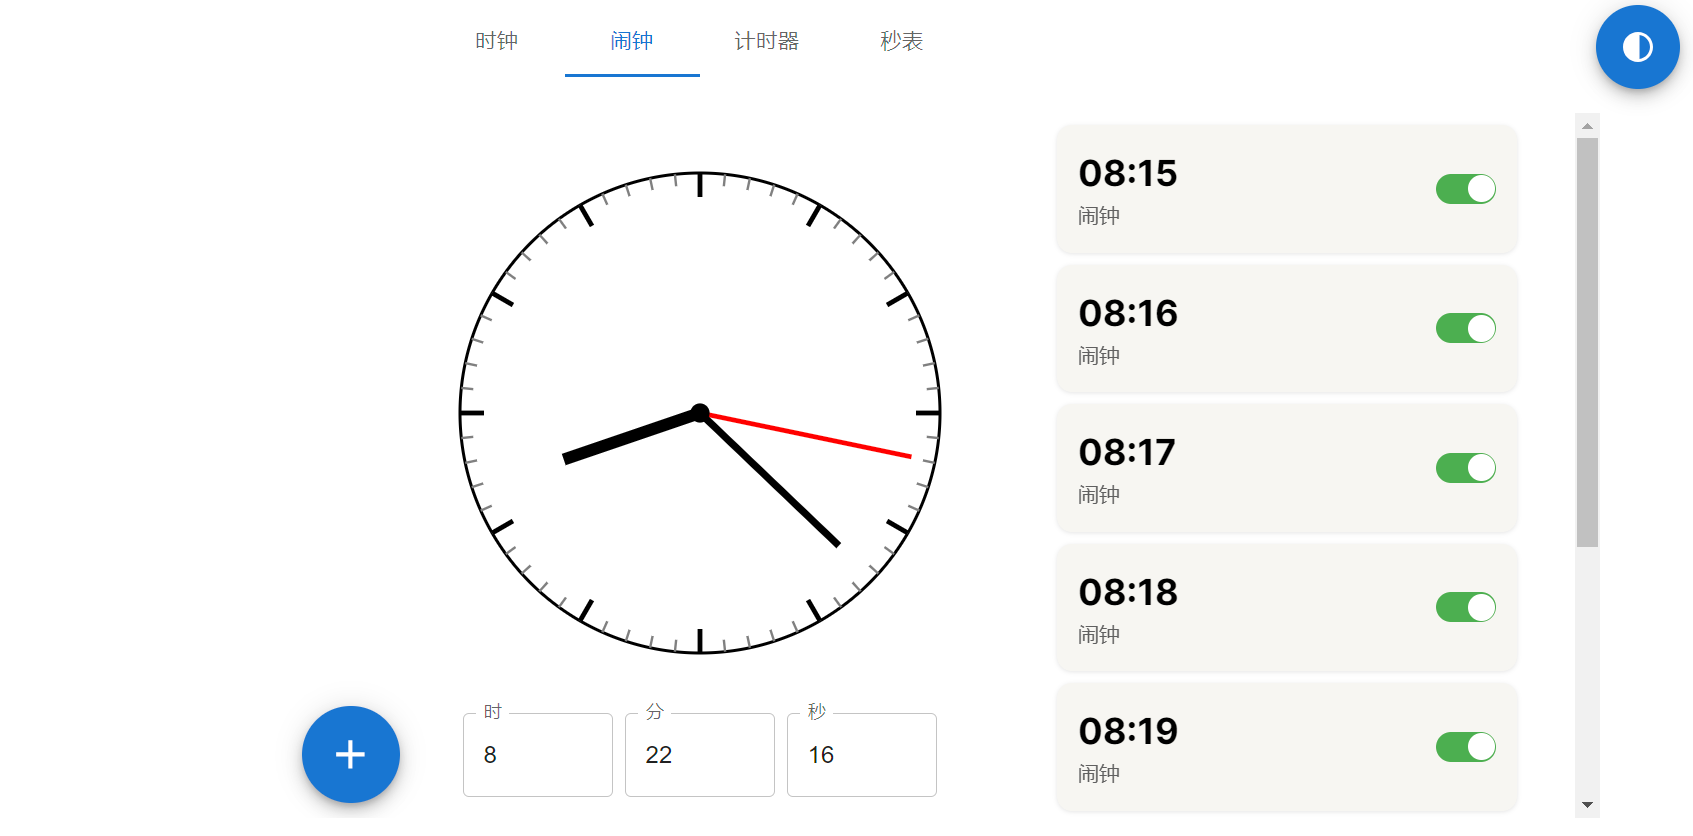
\includegraphics[width=\linewidth]{image/alarm.png}
        \caption{alarm}
            \label{fig:alarm}
    \end{minipage}\hfill
    \begin{minipage}{0.48\textwidth}
        \centering
        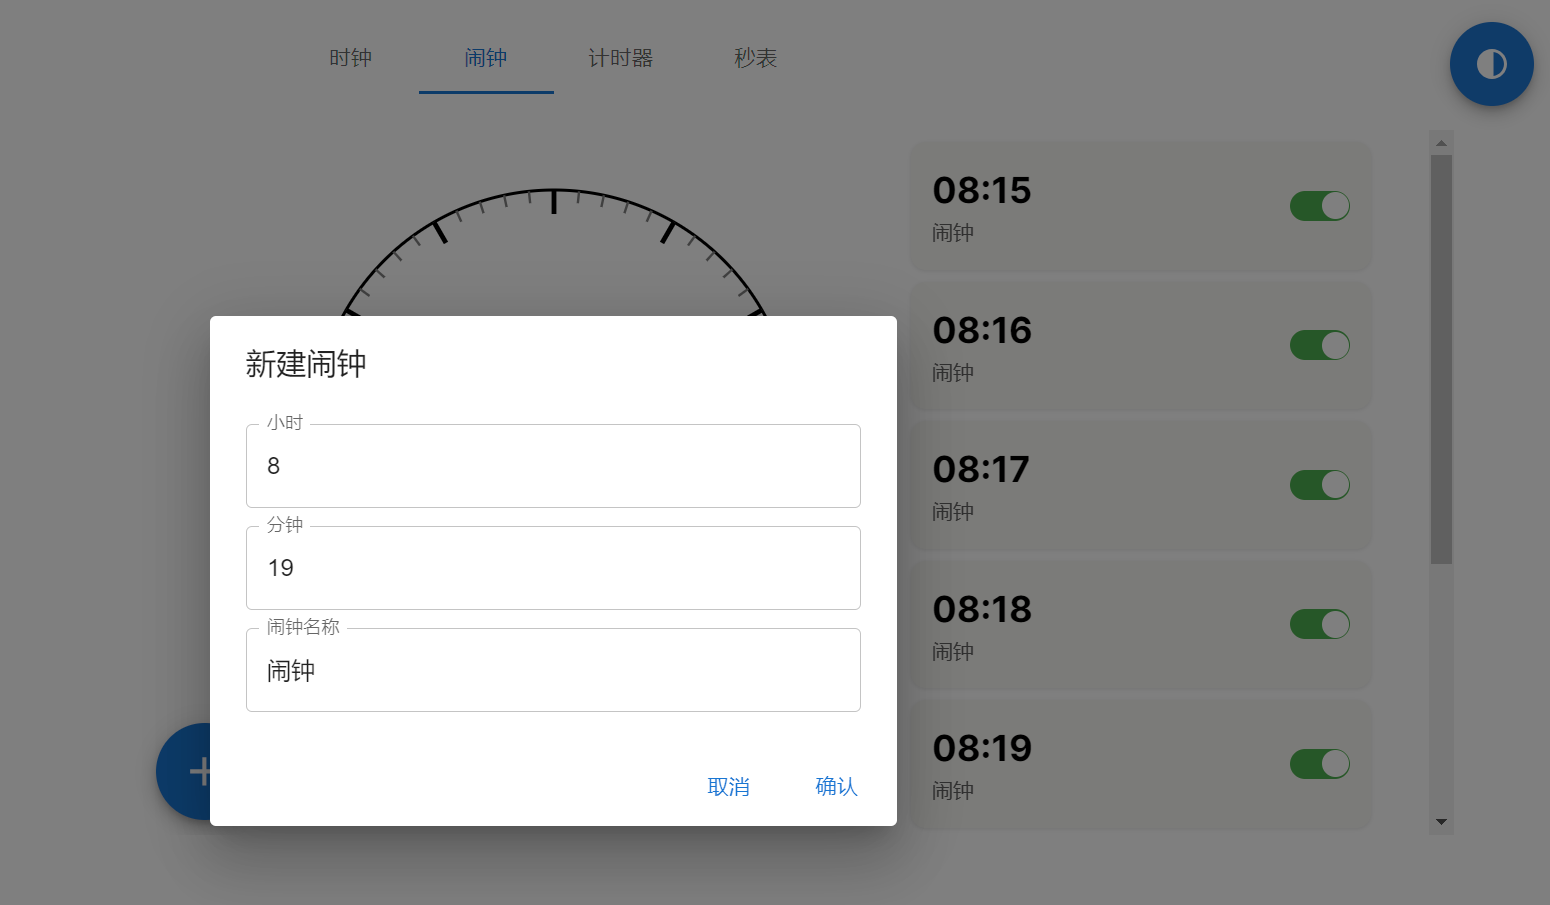
\includegraphics[width=\linewidth]{image/alarm_add.png}
        \caption{alarm\_add}
        \label{fig:alarm_add}
    \end{minipage}
\end{figure}

\subsubsection{编辑闹钟}
在图\ref{fig:alarm}中,点击右方闹钟处的滑动开关可控制闹钟的开启与关闭

直接点击闹钟可进入图\ref{fig:alarm_edit}进行闹钟编辑,包含“更改时间”以及“删除闹钟”功能
\subsubsection{闹钟响起}\label{subsec:alarm}
当到达某一闹钟设置的时间后,将会显示图\ref{fig:alarm_tri},弹出两个通知,分别为界面通知和系统通知,

\begin{itemize}
  \item 界面通知:即图\ref{fig:alarm_tri}正中间的通知,可显示距离闹钟响起过去了多长时间,点击界面的任意处即可关闭。
  \item 系统通知:即图\ref{fig:alarm_tri}右下角的通知,点击后可以回到闹钟界面。
\end{itemize}

\begin{figure}[!h]
    \centering
    \begin{minipage}{0.48\textwidth}
        \centering
        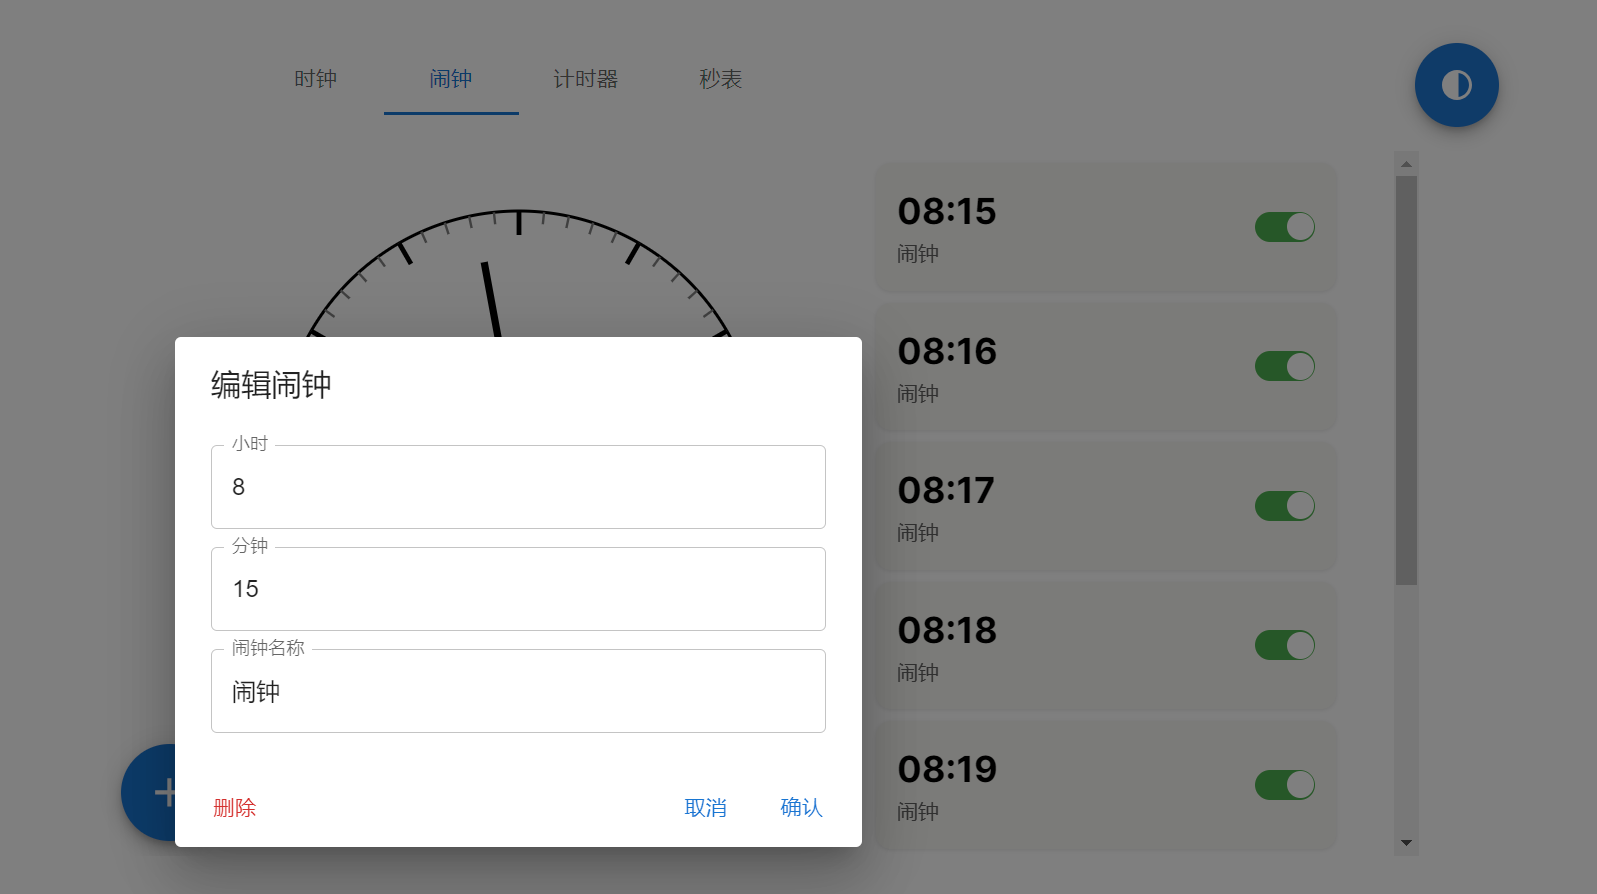
\includegraphics[width=\linewidth]{image/alarm_edit.png}
        \caption{alarm\_edit}
            \label{fig:alarm_edit}
    \end{minipage}\hfill
    \begin{minipage}{0.48\textwidth}
        \centering
        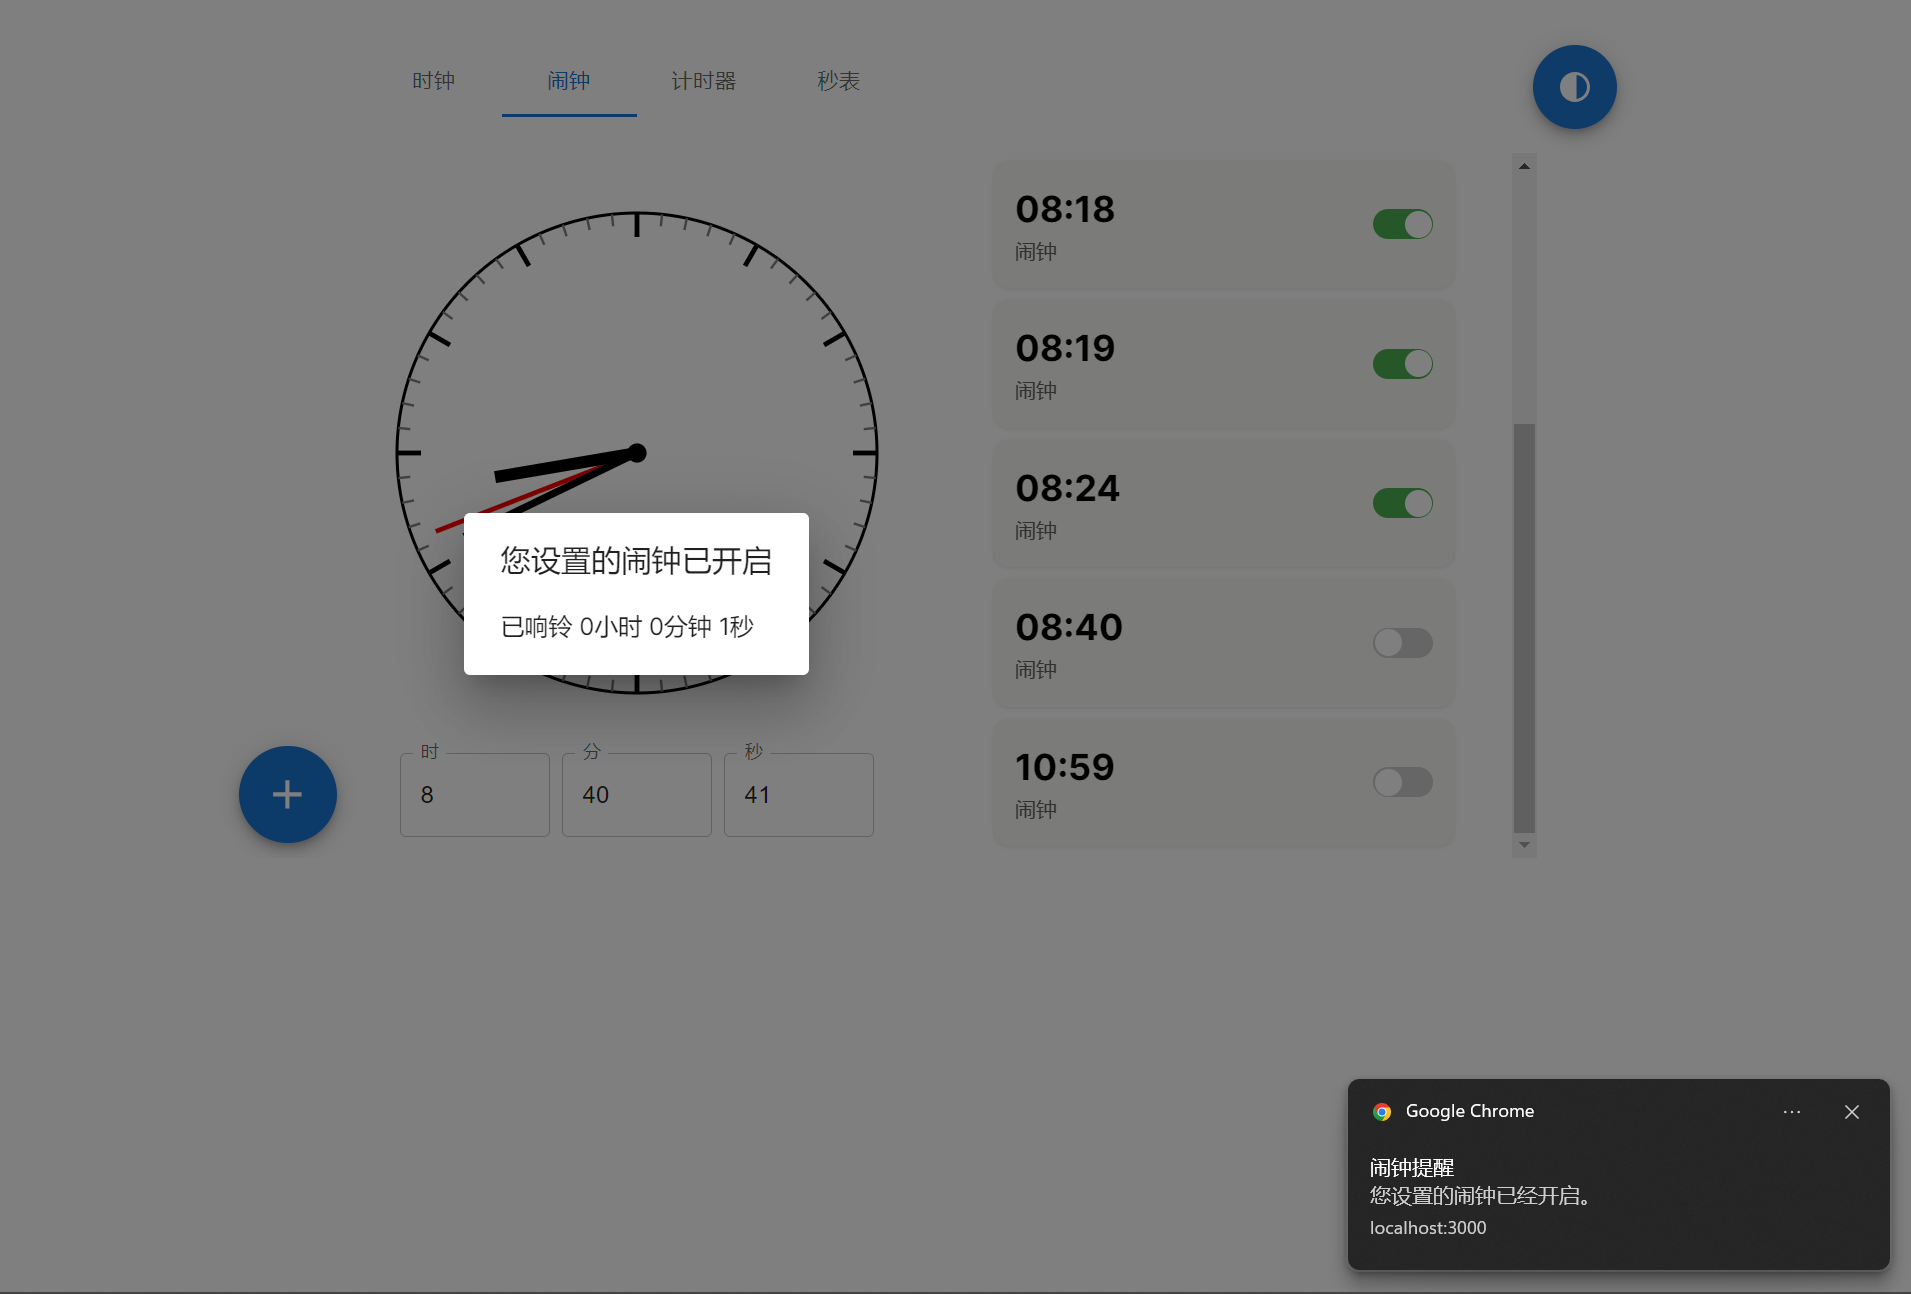
\includegraphics[width=\linewidth]{image/alarm_trigger.png}
        \caption{alarm\_tri}
        \label{fig:alarm_tri}
    \end{minipage}
\end{figure}


\subsection{计时器}
\subsubsection{计时功能}
在图\ref{fig:timer}中,点击“编辑”按钮即可编辑计时器的时间,“恢复”和“暂停”按钮可控制计时器的开启与关闭。
\subsubsection{计时器响起}
计时器时间归零后,进入图\ref{fig:timer_tri},弹出两个通知,分别为界面通知和系统通知,与 \ref{subsec:alarm}中功能相同。

\begin{figure}[!h]
    \centering
    \begin{minipage}{0.48\textwidth}
        \centering
        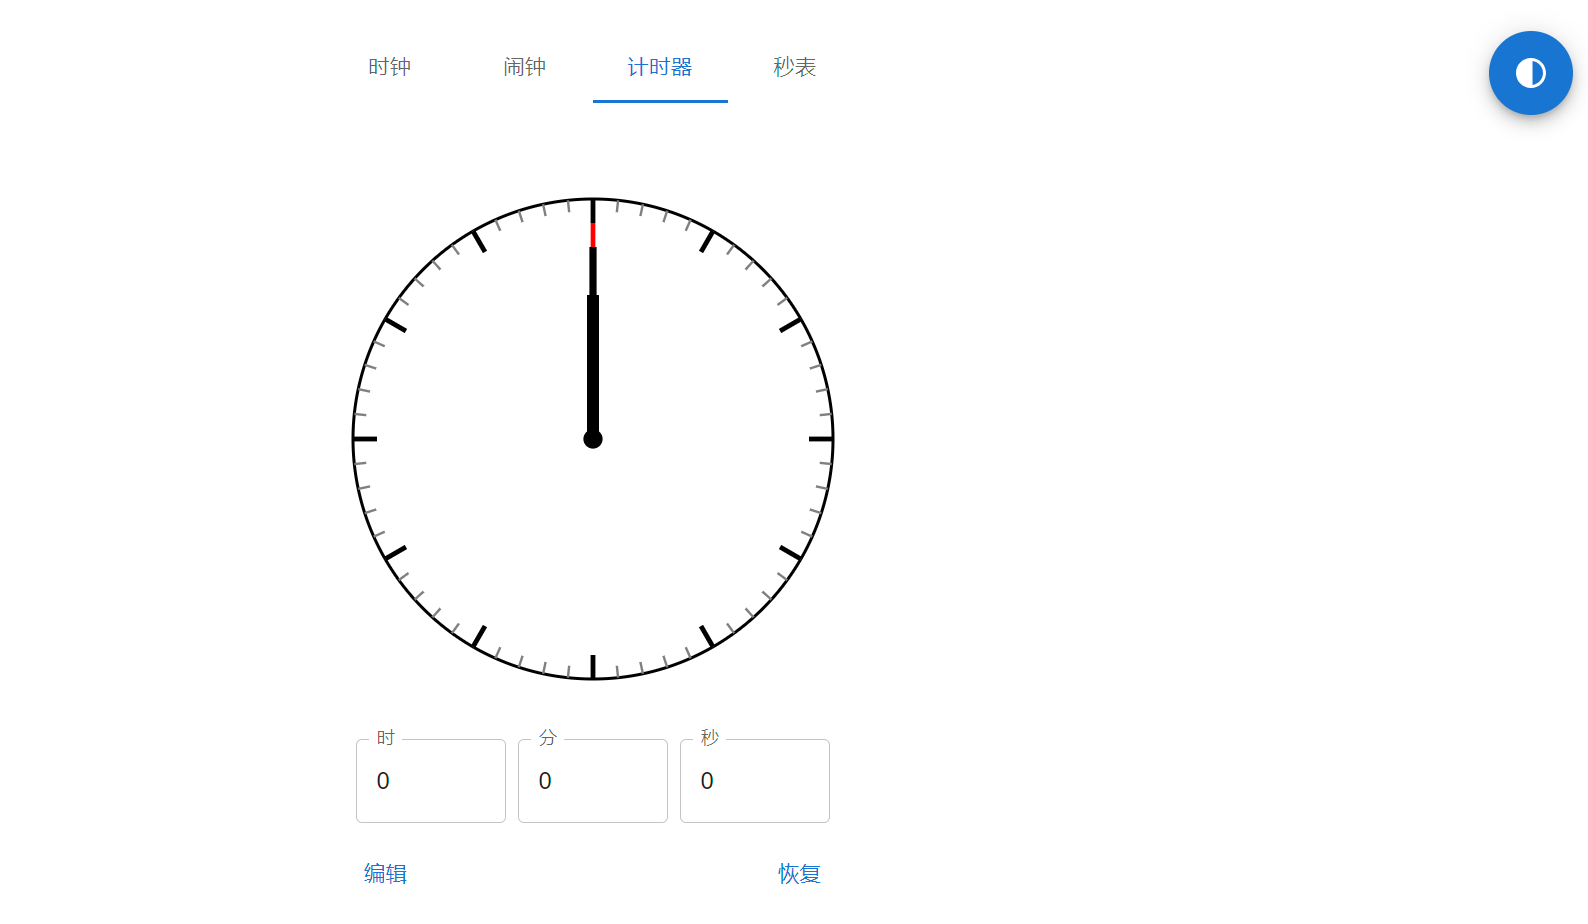
\includegraphics[width=\linewidth]{image/timer.png}
        \caption{timer}
            \label{fig:timer}
    \end{minipage}\hfill
    \begin{minipage}{0.48\textwidth}
        \centering
        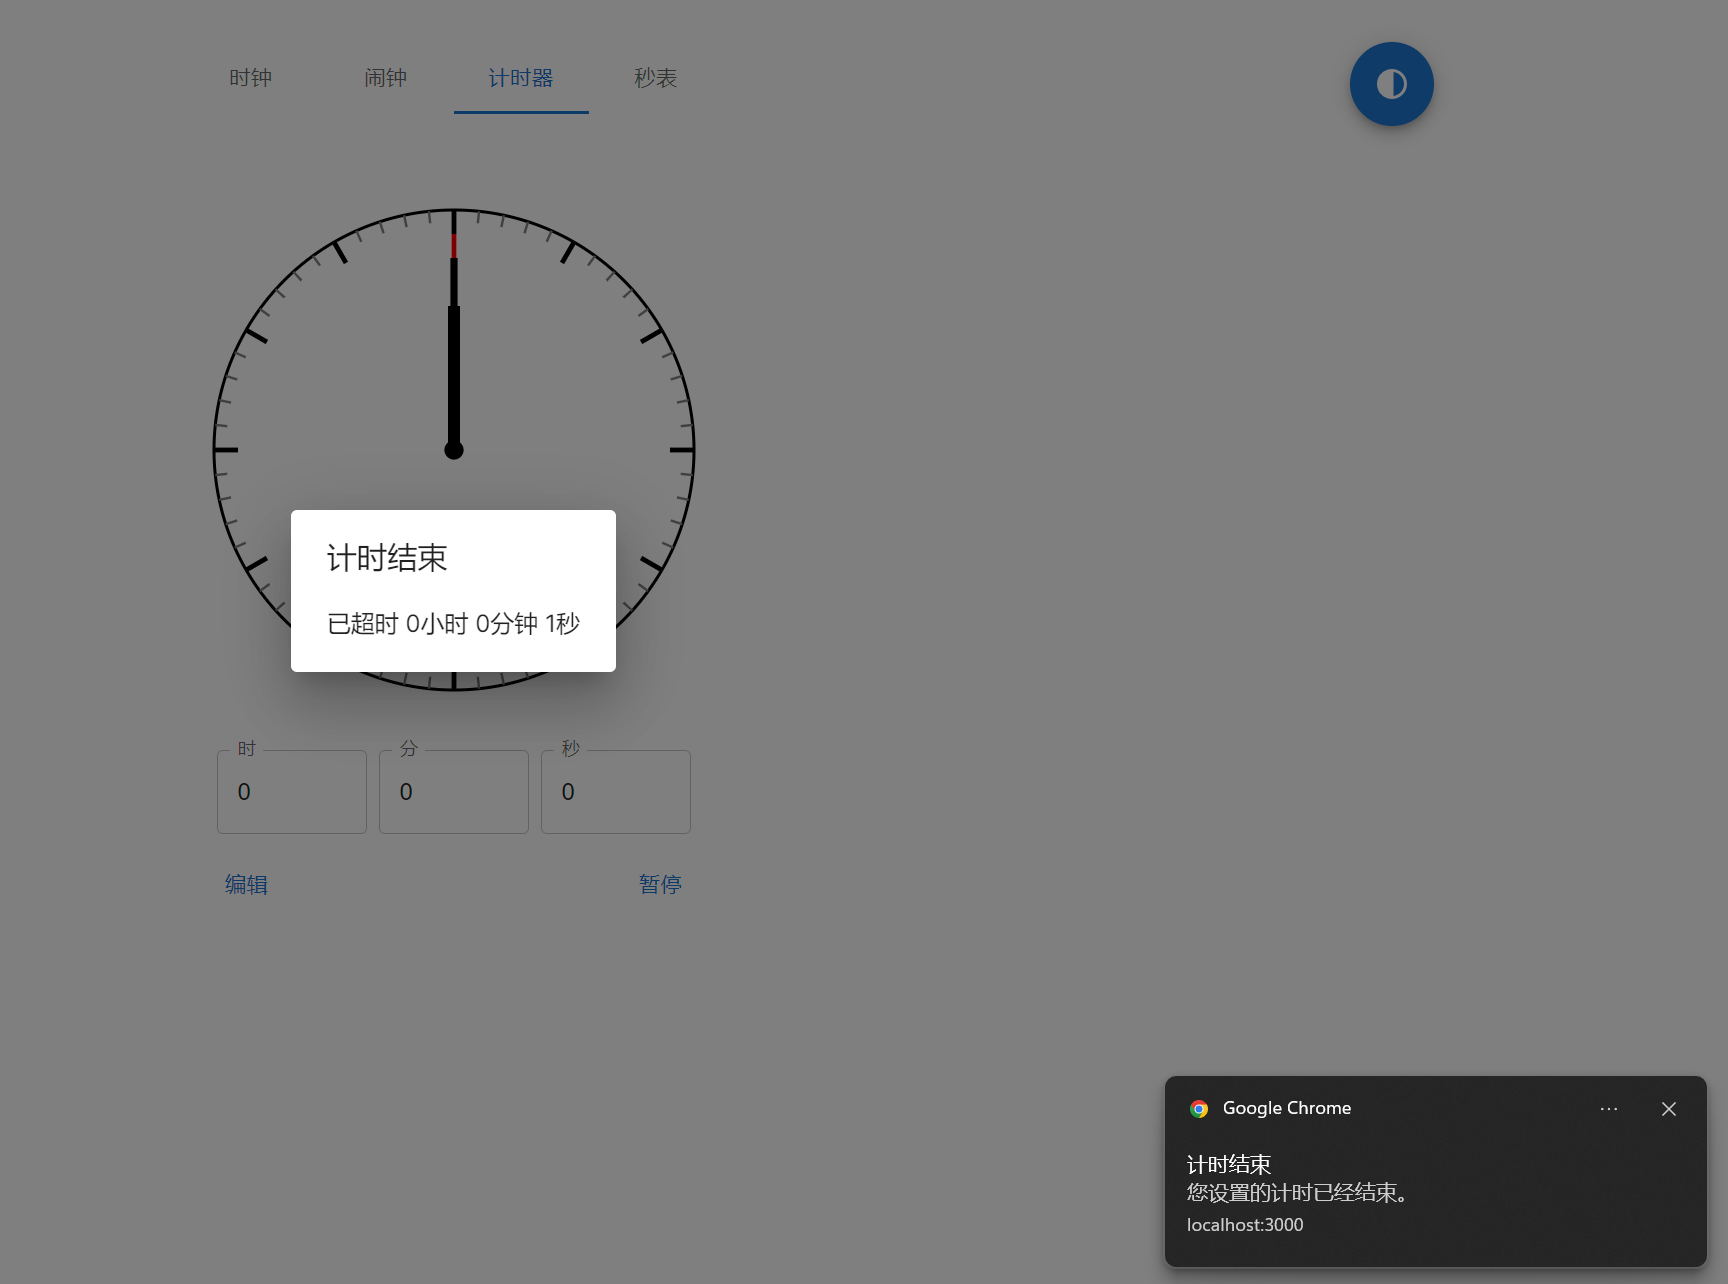
\includegraphics[width=\linewidth]{image/timer_tri.png}
        \caption{timer\_tri}
        \label{fig:timer_tri}
    \end{minipage}
\end{figure}

\subsection{秒表}
\subsubsection{计时功能}
在图\ref{fig:stopwatch}中,点击“启动”按钮即可开始计时,开始计时后可通过“暂停”和“复位”按钮来停止计时和重置计时。
\subsubsection{标记功能}
在开始计时后,可点击“标记”按钮来记录时间,效果如图\ref{fig:stopwatch_time},在点击“复位”后记录消失。

\begin{figure}[!h]
    \centering
    \begin{minipage}{0.48\textwidth}
        \centering
        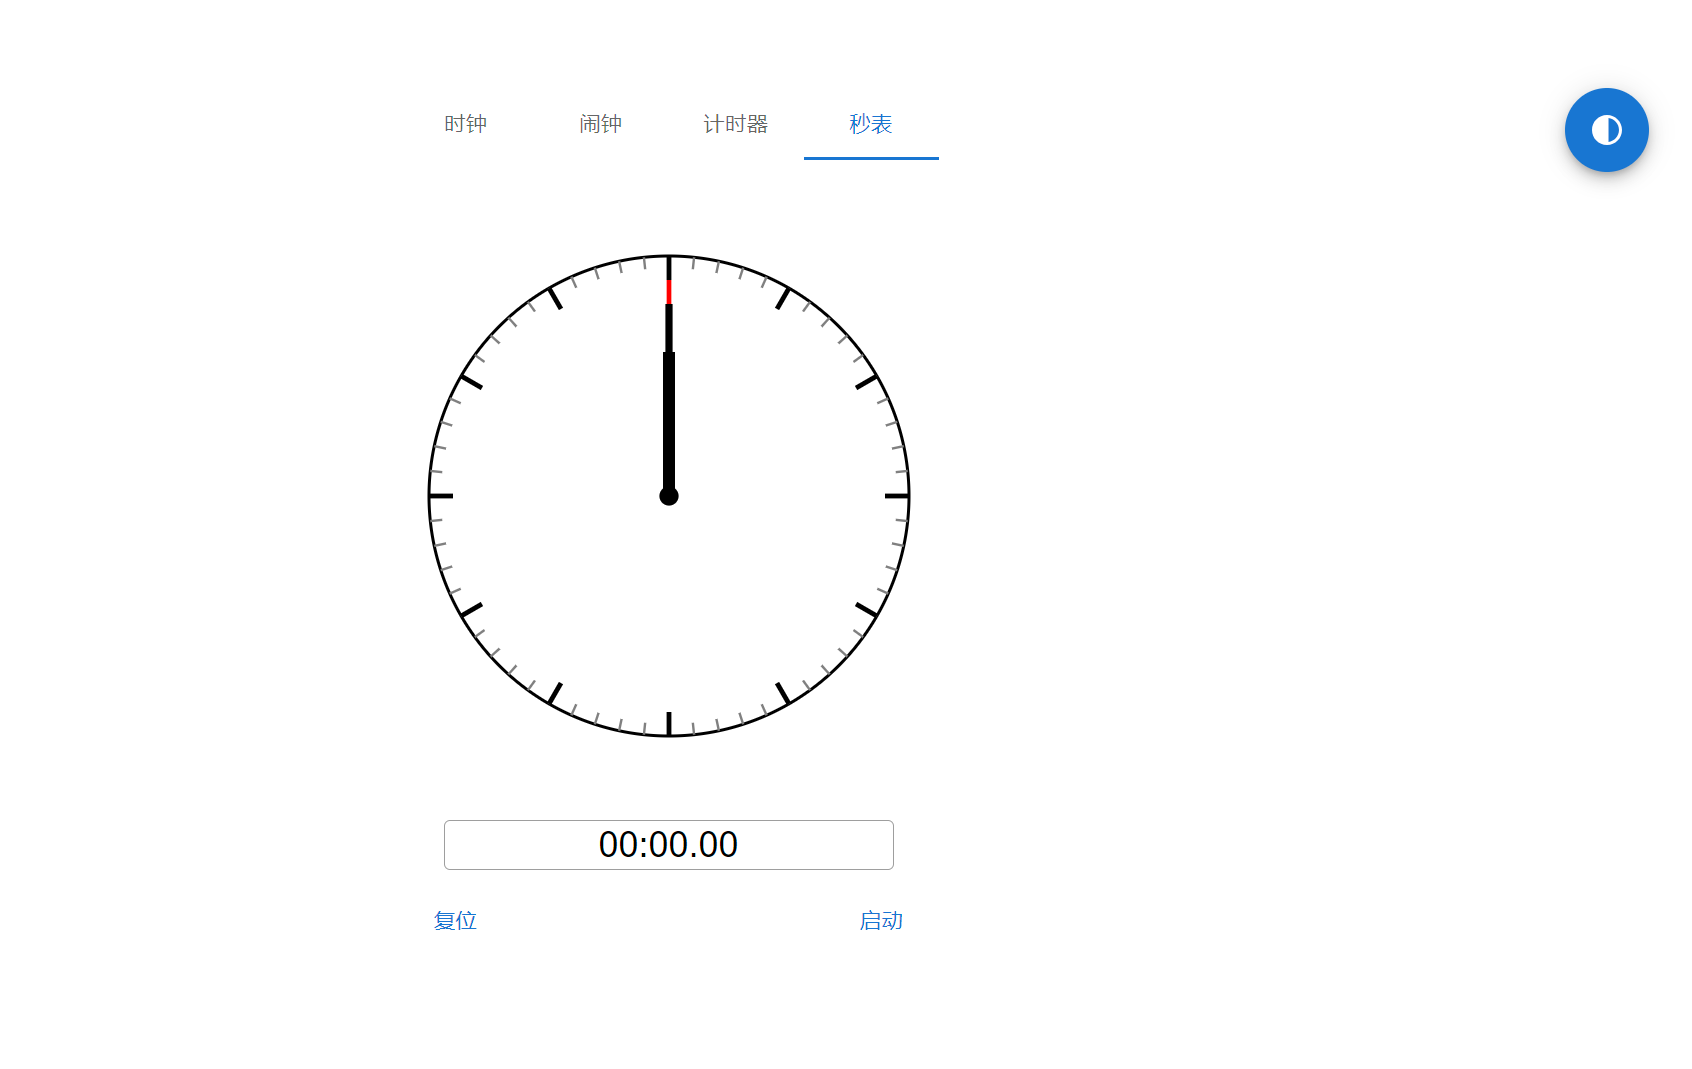
\includegraphics[width=\linewidth]{image/stopwatch.png}
        \caption{stopwatch}
            \label{fig:stopwatch}
    \end{minipage}\hfill
    \begin{minipage}{0.48\textwidth}
        \centering
        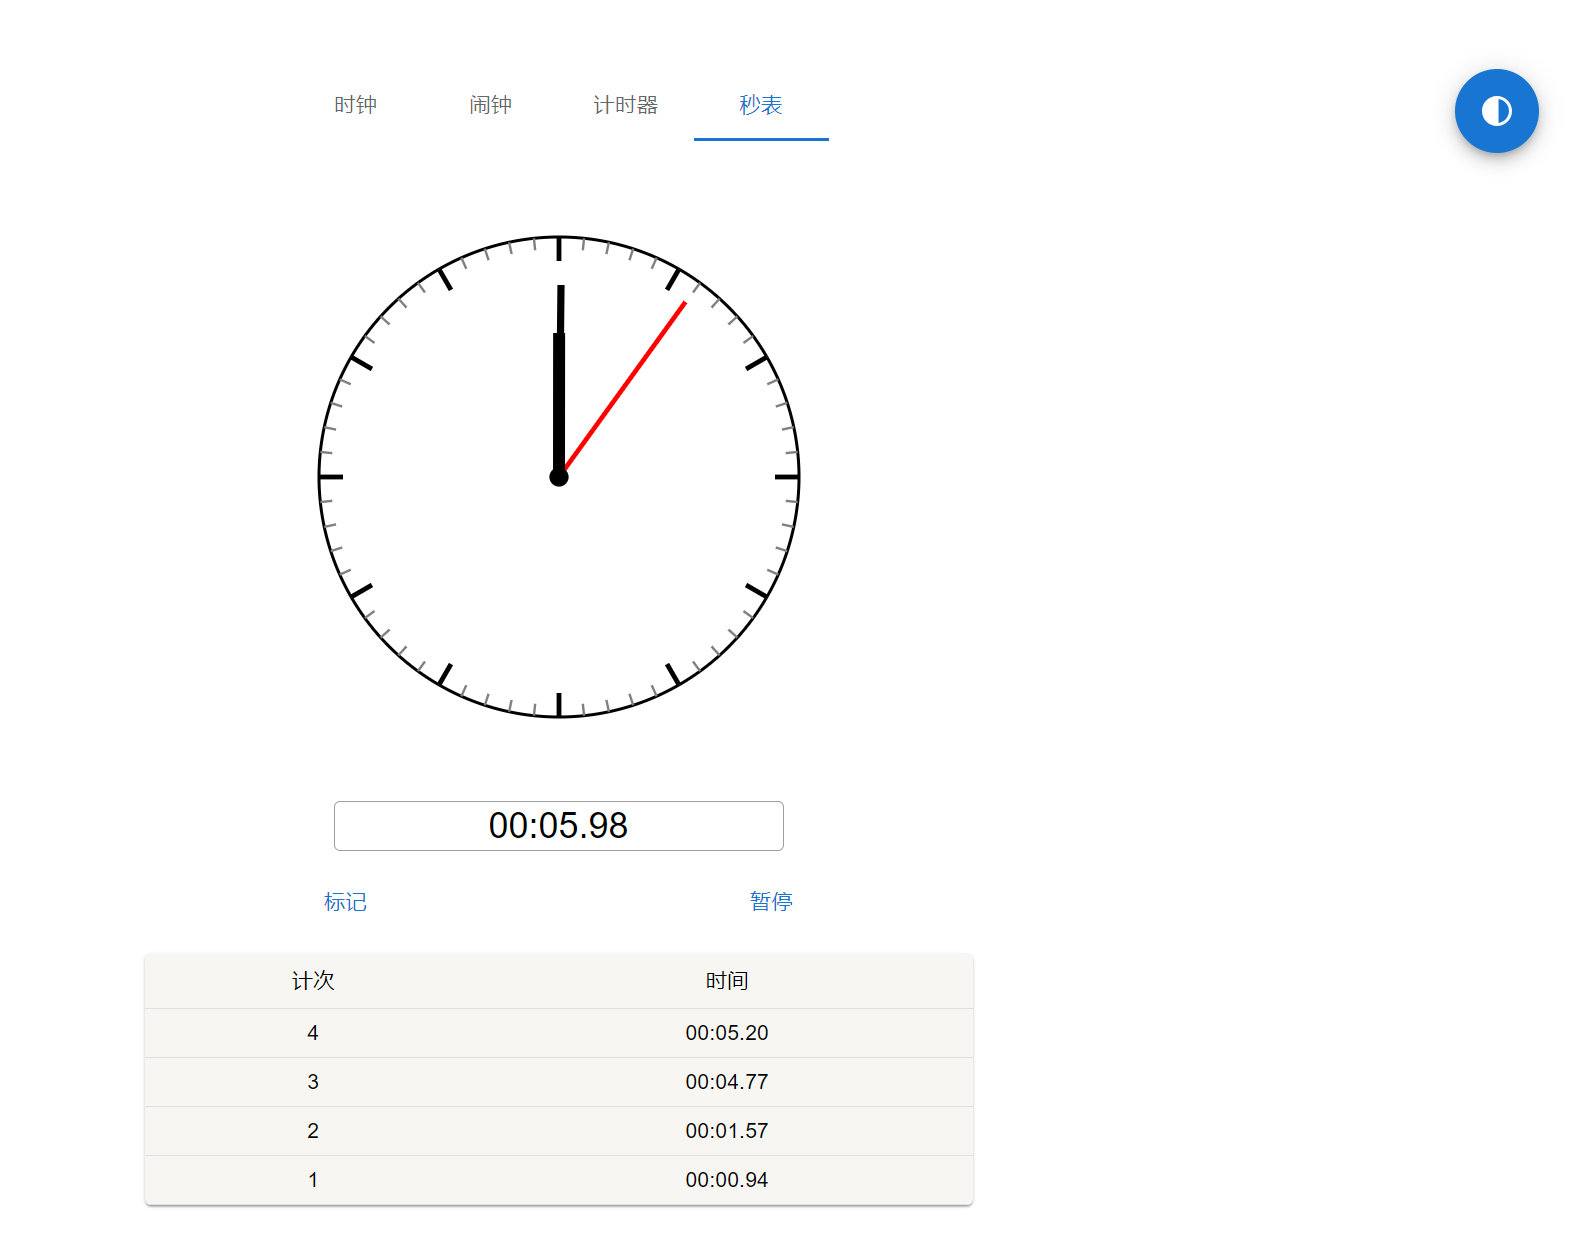
\includegraphics[width=\linewidth]{image/stopwatch_time.png}
        \caption{stopwatch\_time}
        \label{fig:stopwatch_time}
    \end{minipage}
\end{figure}

\subsection{明暗模式切换}
在每个界面的右上角存在“明暗模式切换按钮”,点击可更改为明亮或是黑暗模式,下面为效果对比图

\begin{figure}[!h]
    \centering
    \begin{minipage}{0.48\textwidth}
        \centering
        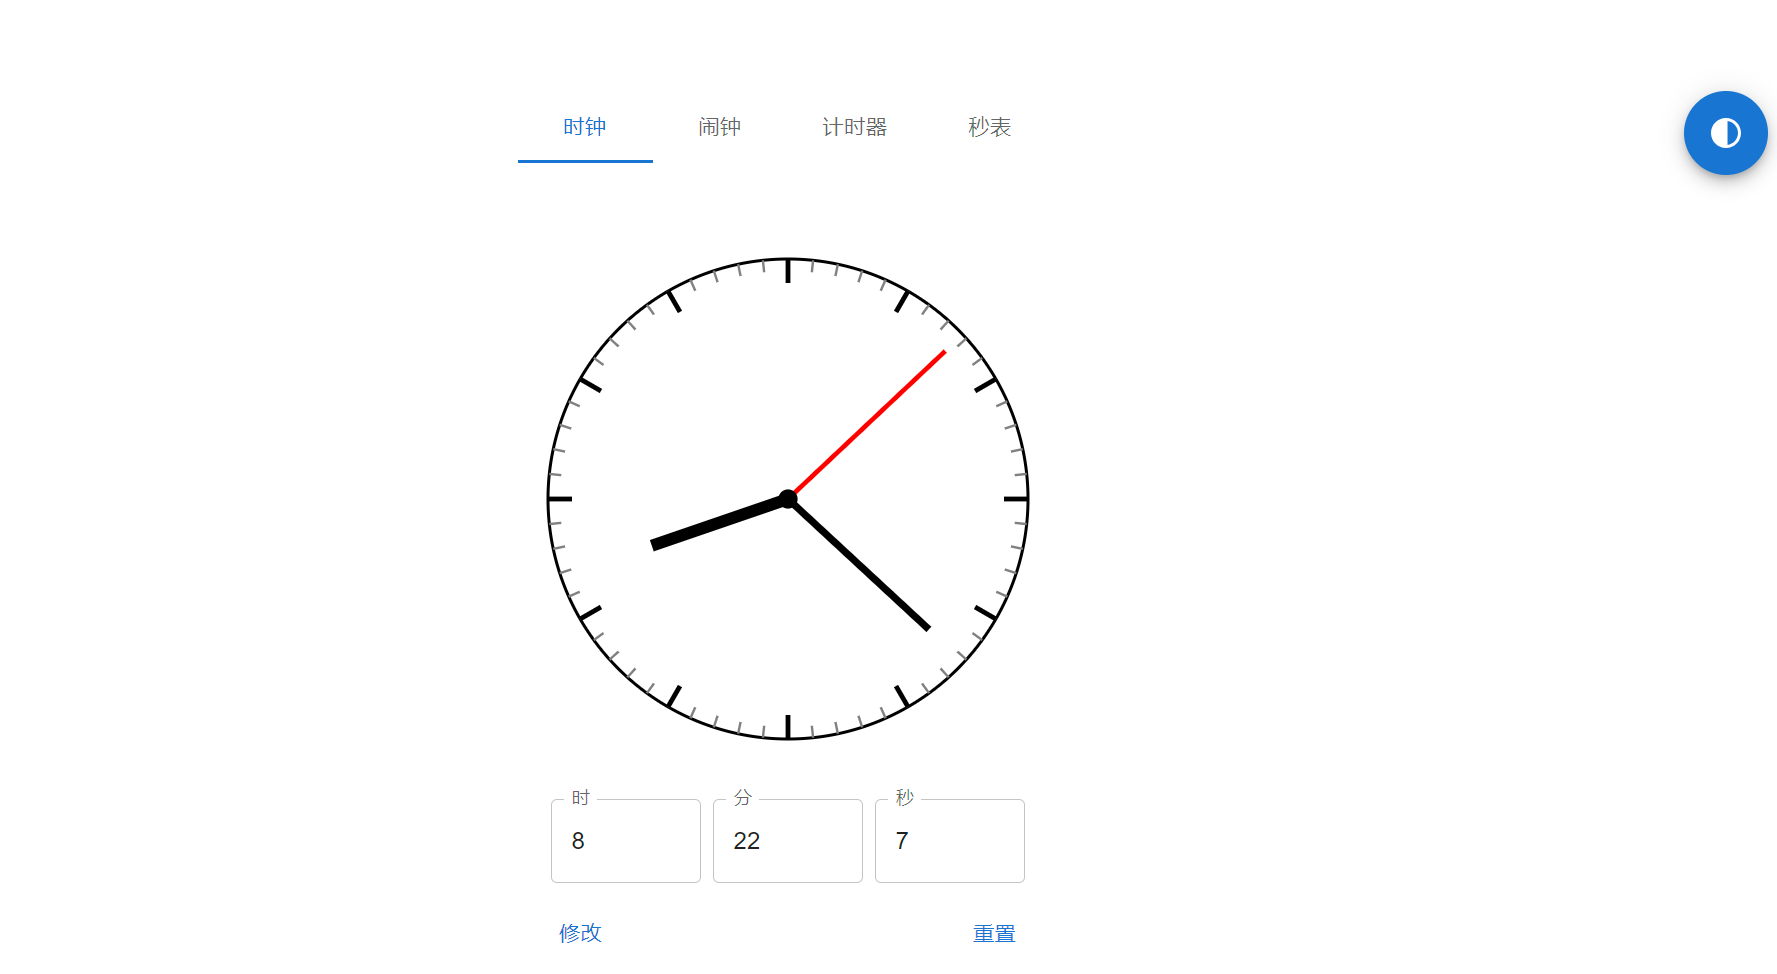
\includegraphics[width=\linewidth]{image/clock.png}
        \caption{clock\_light}
    \end{minipage}\hfill
    \begin{minipage}{0.48\textwidth}
        \centering
        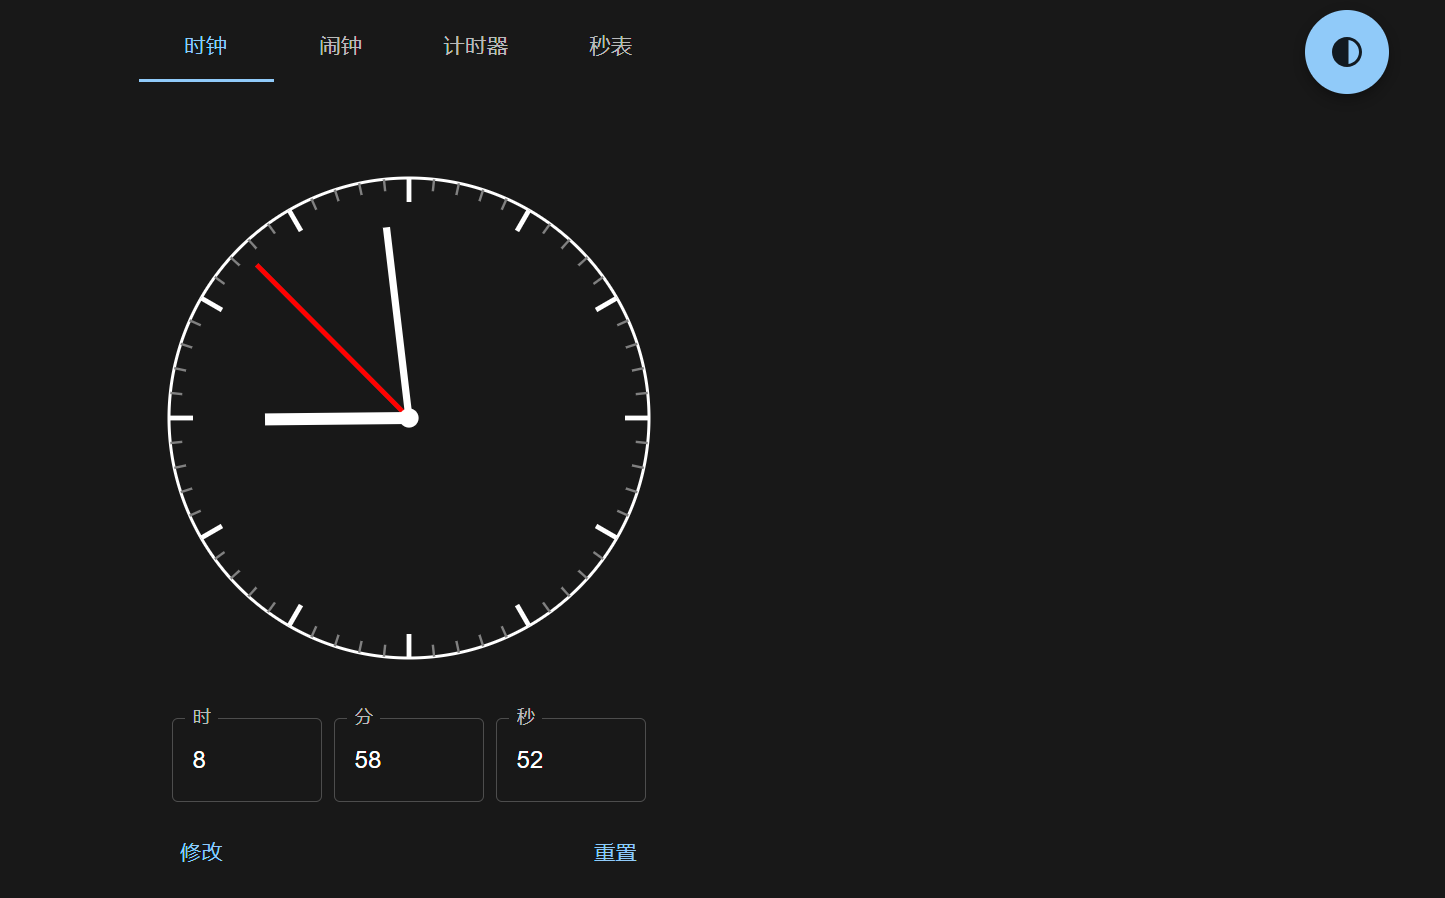
\includegraphics[width=\linewidth]{image/clock_black.png}
        \caption{clock\_black}
    \end{minipage}\hfill
    \begin{minipage}{0.48\textwidth}
        \centering
        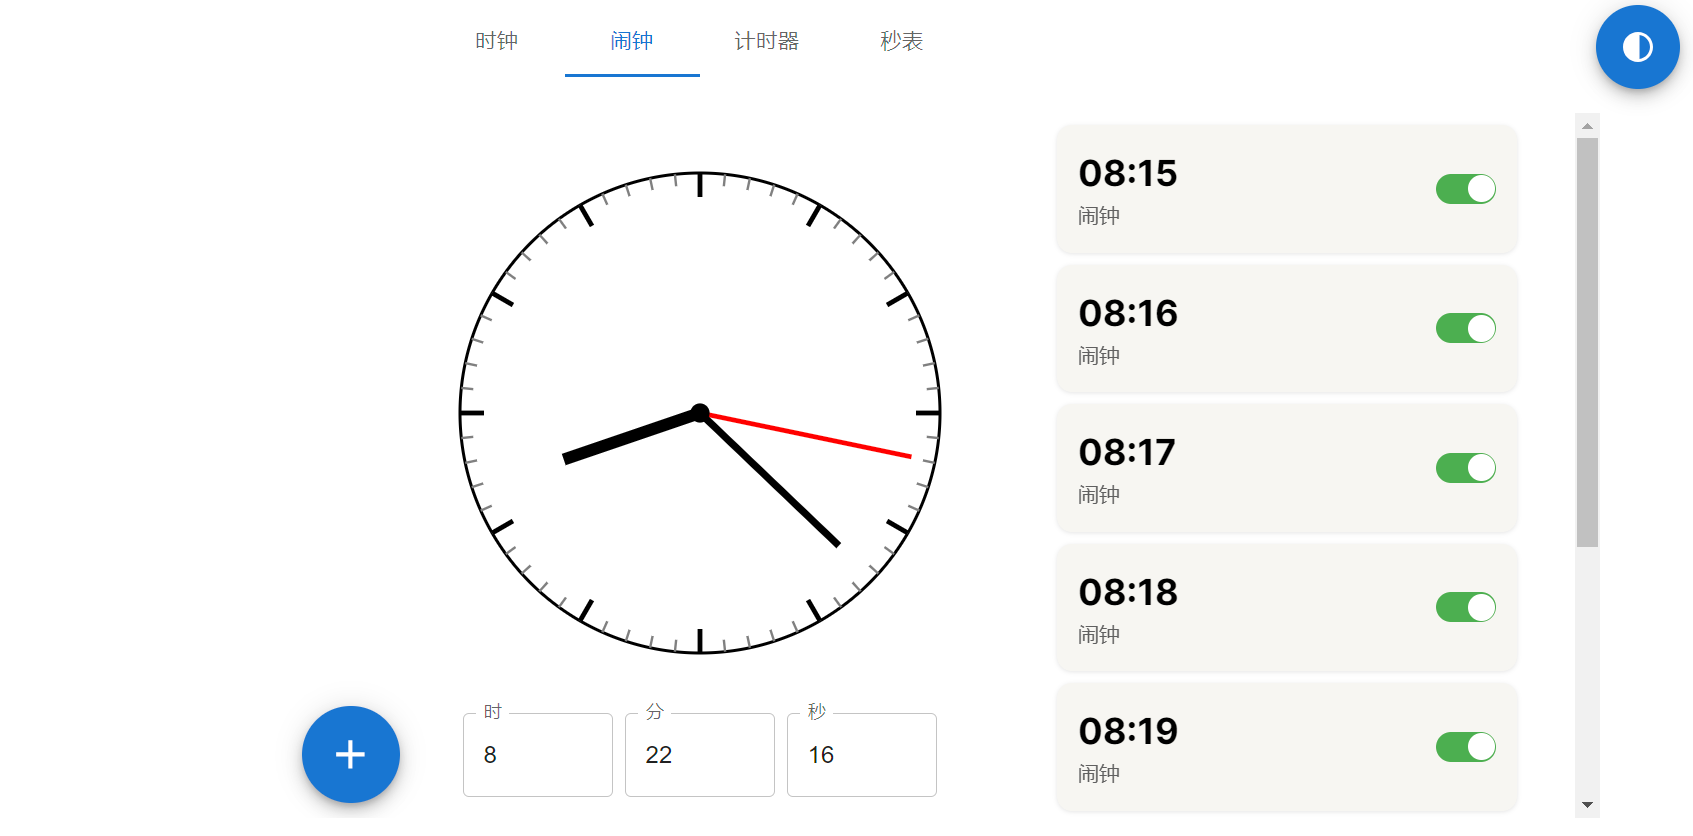
\includegraphics[width=\linewidth]{image/alarm.png}
        \caption{alarm\_light}
    \end{minipage}\hfill
    \begin{minipage}{0.48\textwidth}
        \centering
        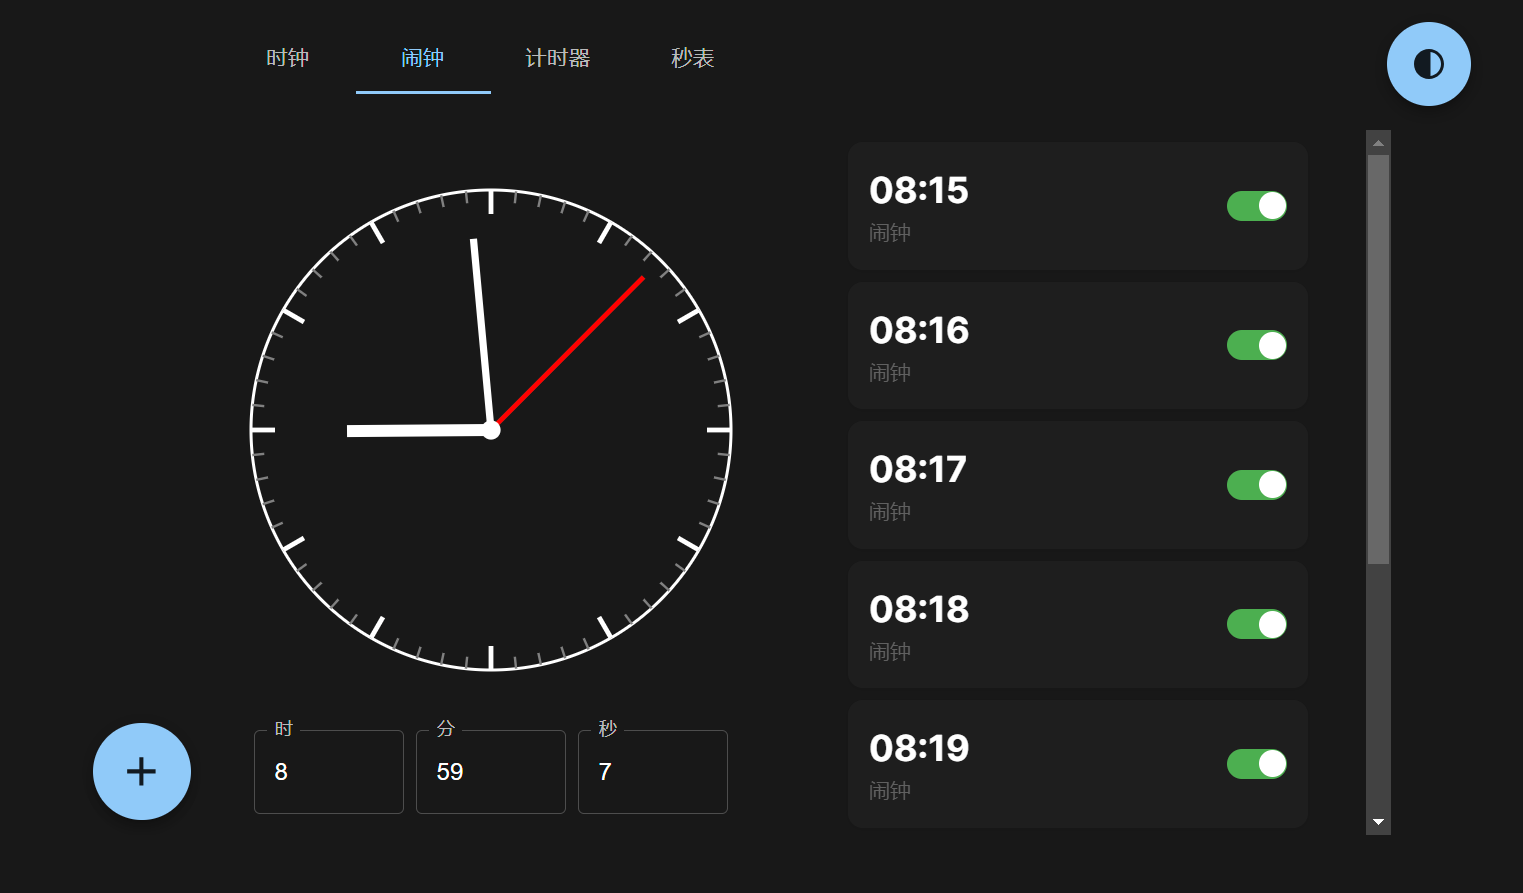
\includegraphics[width=\linewidth]{image/alarm_black.png}
        \caption{alarm\_black}
    \end{minipage}\hfill
    
\end{figure}
\begin{figure}[!h]
    \begin{minipage}{0.48\textwidth}
        \centering
        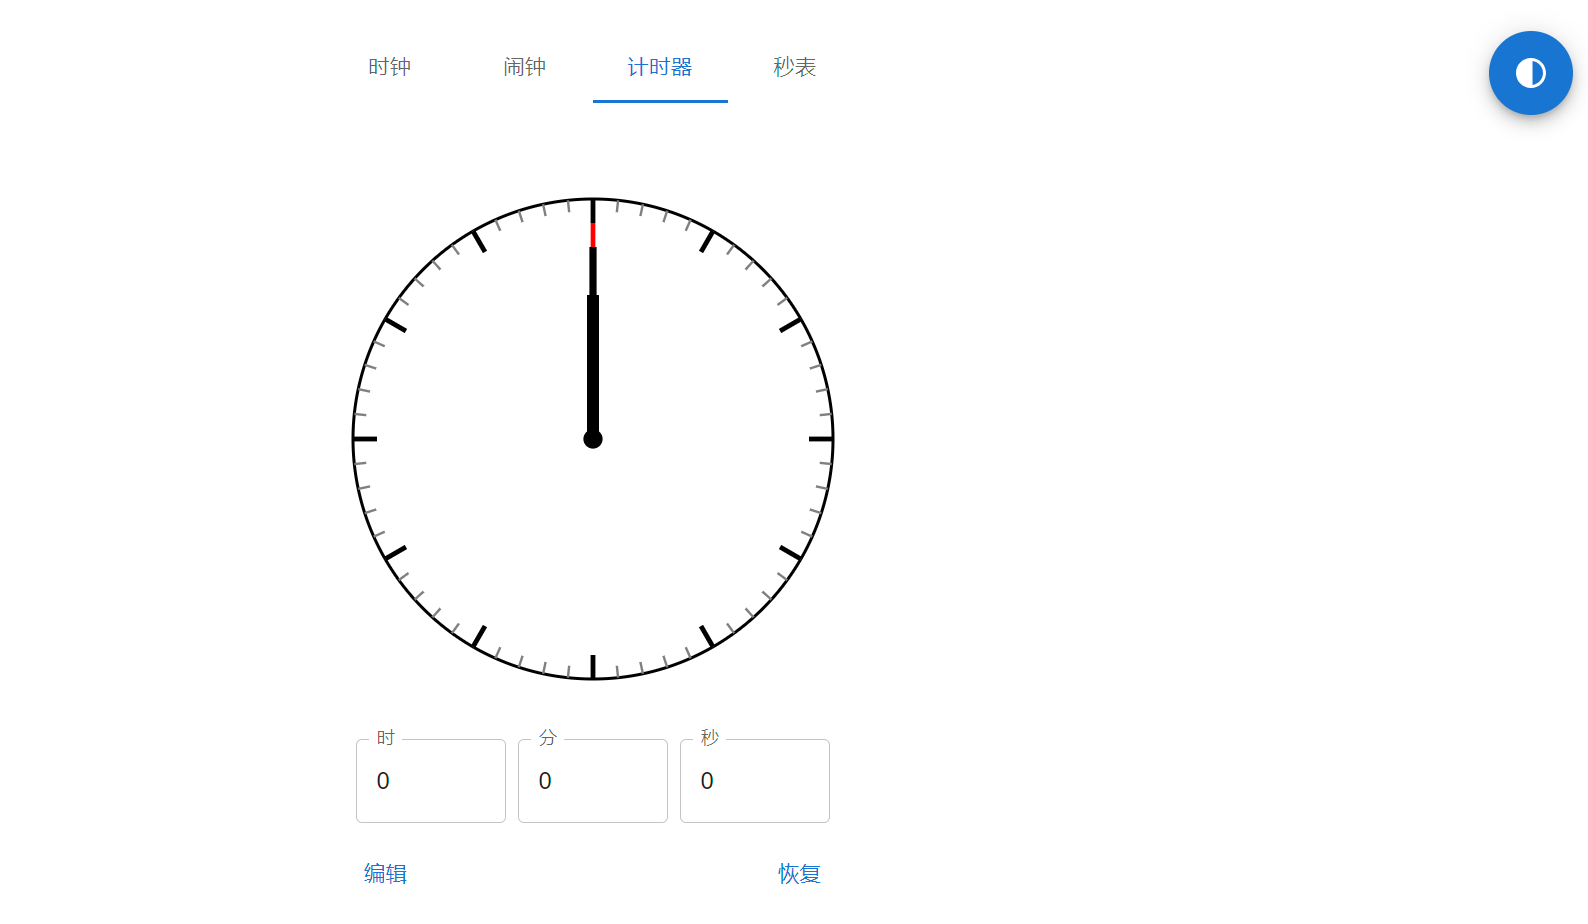
\includegraphics[width=\linewidth]{image/timer.png}
        \caption{timer\_light}
    \end{minipage}\hfill
    \begin{minipage}{0.48\textwidth}
        \centering
        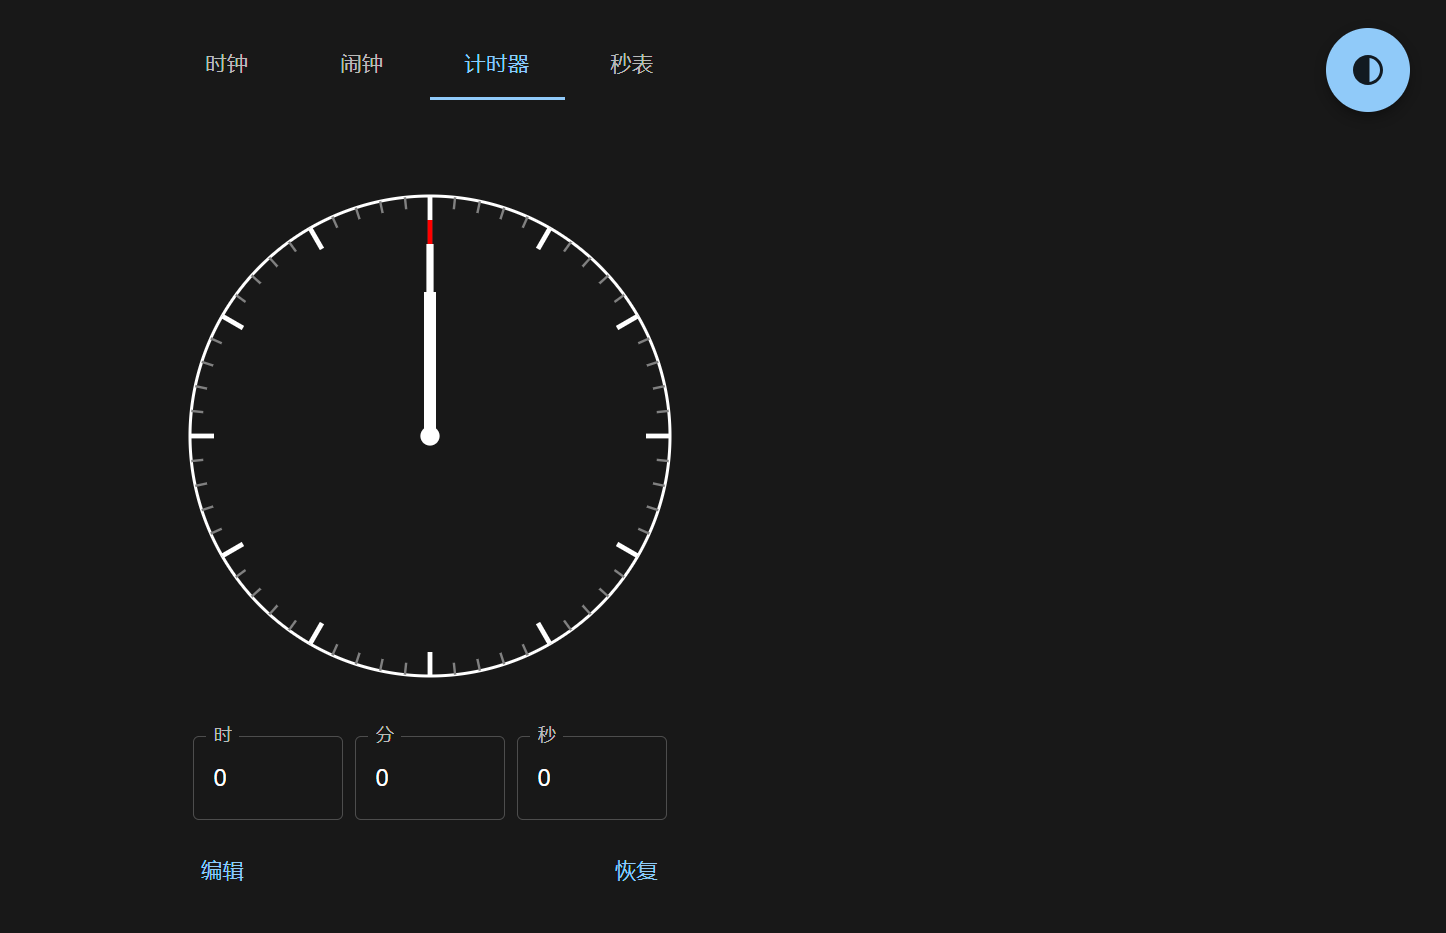
\includegraphics[width=\linewidth]{image/timer_black.png}
        \caption{timer\_black}
    \end{minipage}\hfill
    \begin{minipage}{0.48\textwidth}
        \centering
        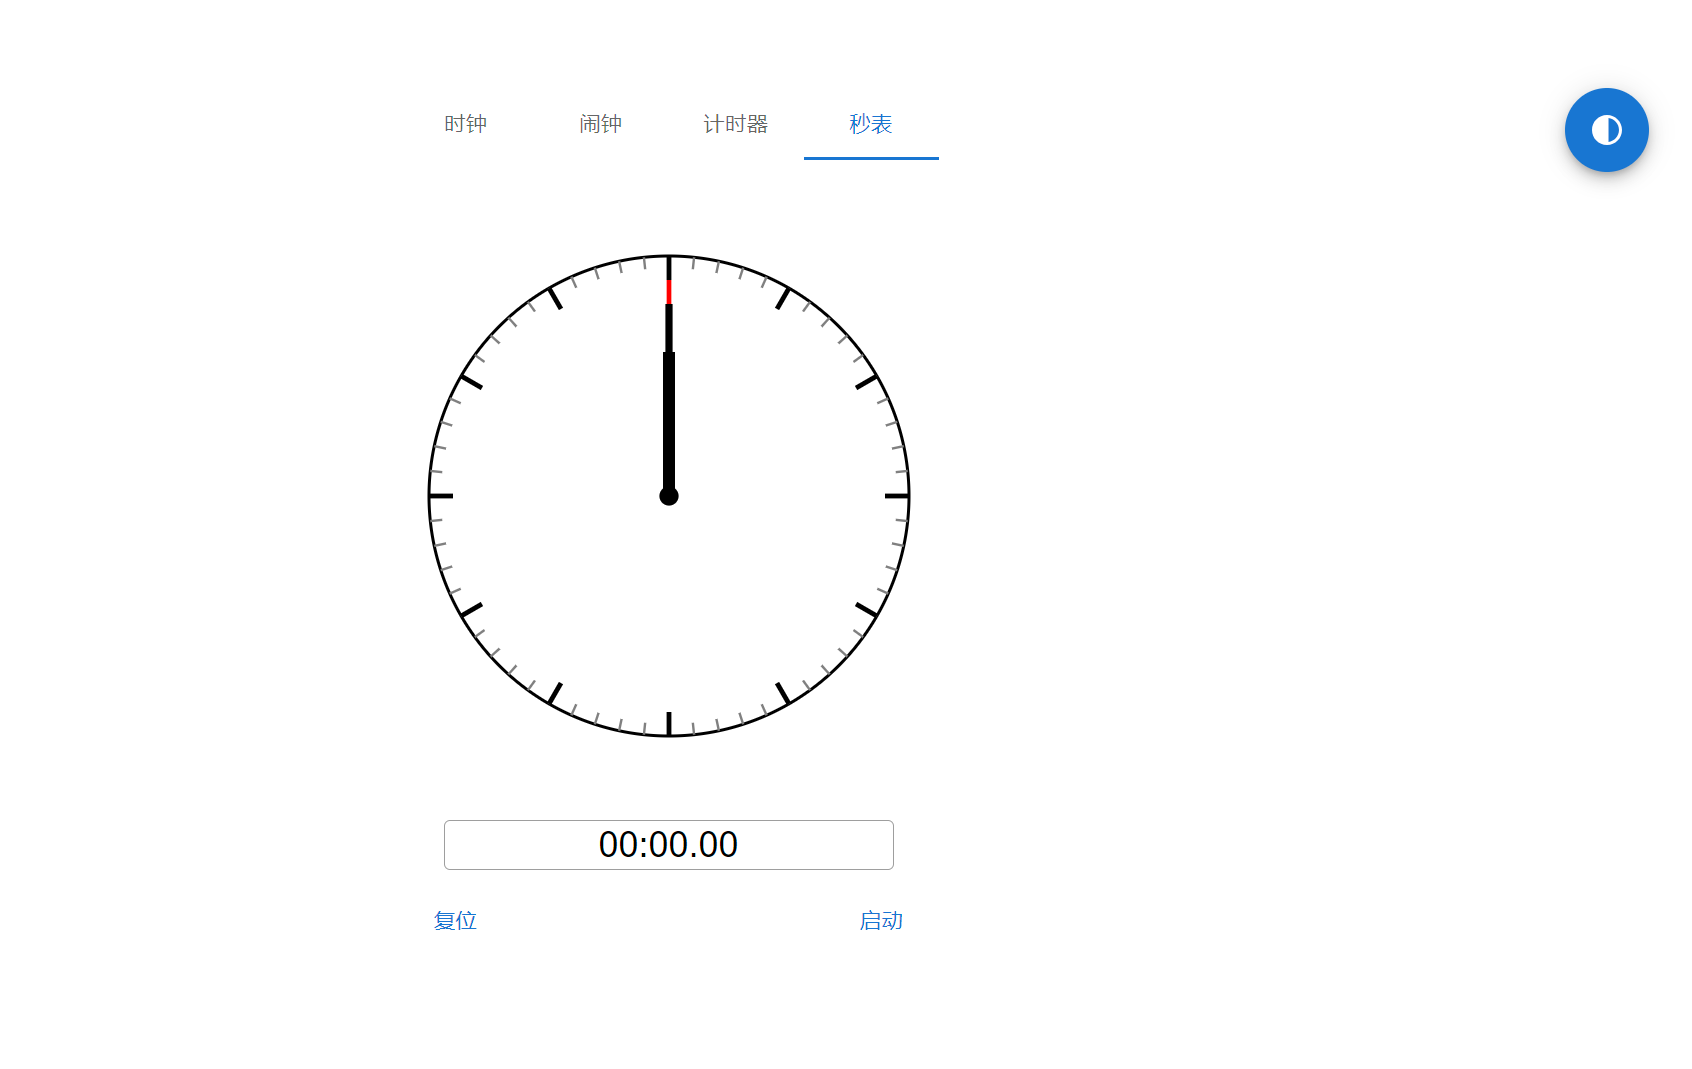
\includegraphics[width=\linewidth]{image/stopwatch.png}
        \caption{stopwatch\_light}
    \end{minipage}
    \begin{minipage}{0.48\textwidth}
        \centering
        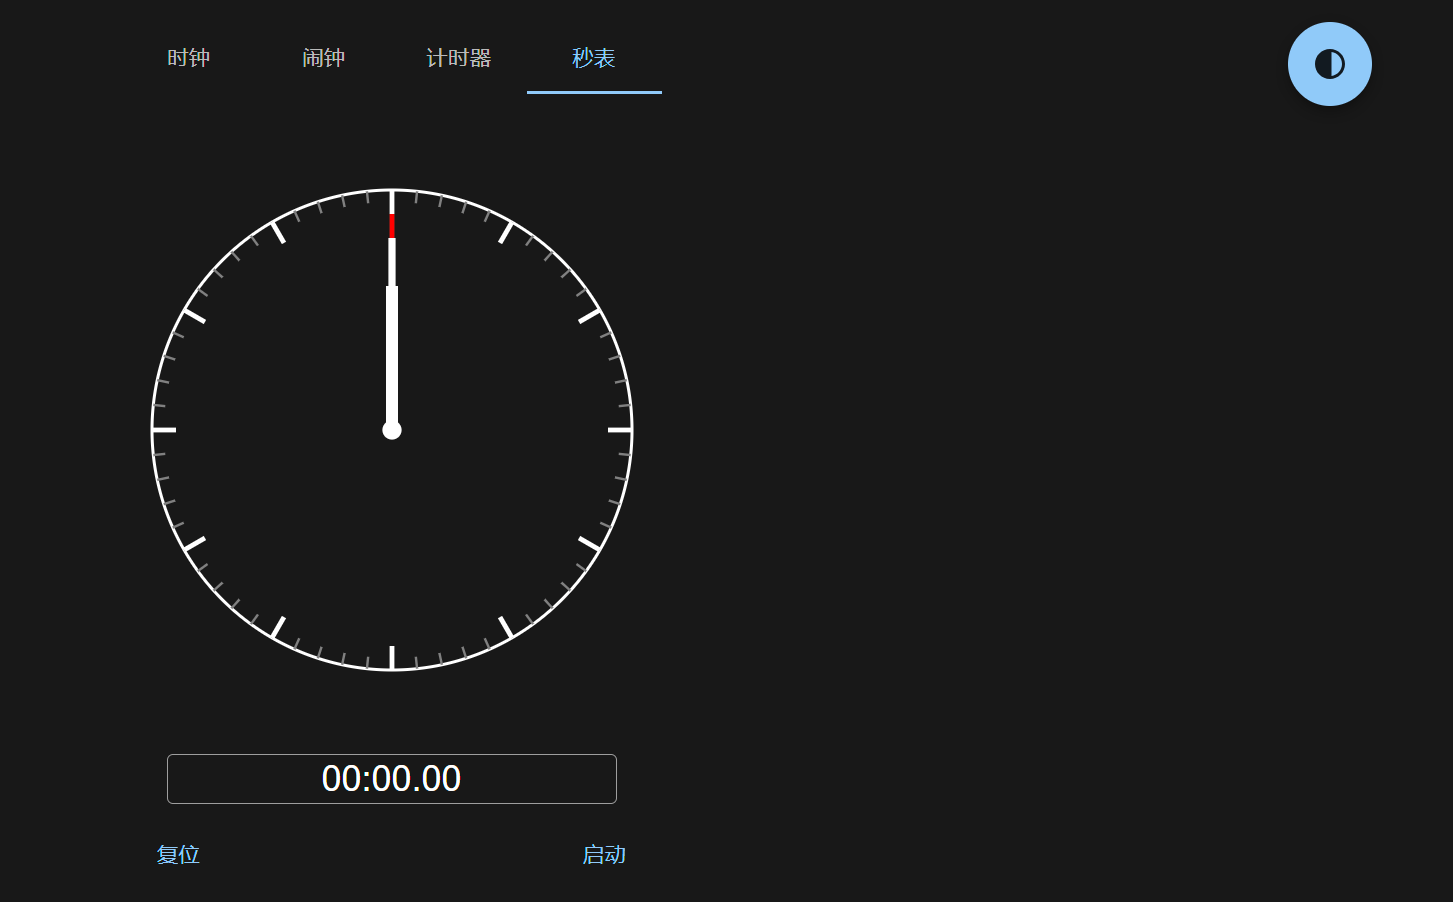
\includegraphics[width=\linewidth]{image/stopwatch_black.png}
        \caption{stopwatch\_black}
    \end{minipage}
\end{figure}
\clearpage
\section{遇到问题及解决办法}
\end{document}
